\section{Contexte et état de l'art}

Les changements climatiques sont devenus un enjeu majeur à l'échelle mondiale, affectant la croissance et la survie des plantes, ainsi que la qualité et la quantité des récoltes agricoles.
Dans ce contexte, il est important d'étudier les flux d'eau dans les plantes afin de comprendre et de réduire le stress hydrique des cultures et ainsi optimiser les productions agricoles dans des climats plus contrastés.

\subsection{Flux hydriques}

Mesurer avec précision le flux hydrique dans les plantes constitue une étape limitante dans l'étude des relations entre le sol et la plante.
Le mécanisme général régissant ces flux au sein des plantes est pourtant aujourd'hui plutôt bien décrit.
\vspace{0.5 cm}

\begin{minipage}{0.5\linewidth}
\captionsetup{type=figure,hypcap=true}
\centering
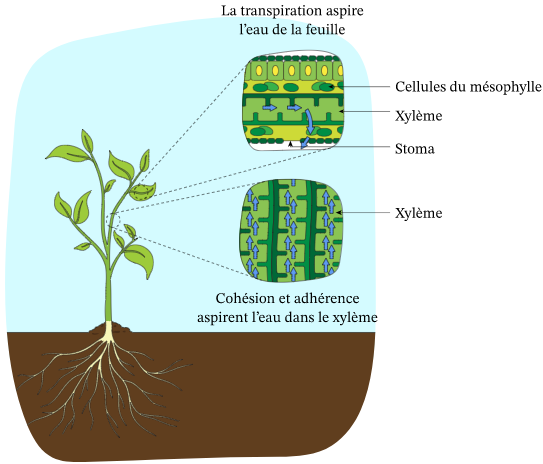
\includegraphics[width=\linewidth]{Image/waterflow_basics.png}
\captionof{figure}{Principe fondamental des flux hydriques dans les plantes \citep{nagwa_fiche_2023}.}
\label{fig:waterflow_basics}
\end{minipage}\hfill
\begin{minipage}{0.45\linewidth}
Comme illustré dans la figure \ref{fig:waterflow_basics}, la perte d'eau par transpiration au travers des stomates des feuilles augmente la tension dans le xylème. Cette tension se propage dans la plante par le principe de cohésion-tension jusque dans les racines.
Lorsque la tension est supérieure à celle du sol environnant, l'eau contenue dans la rhizosphère s'infiltre dans la racine et suit le gradient de potentiel hydrique par les chemins avec le moins de résistance.
Malgré les bonnes définitions des principaux mouvements et facteurs qui interviennent, les flux hydriques à l'échelle de la plante restent toutefois difficilement compréhensibles dans son ensemble \citep{lobet_plant_2014}.
\end{minipage} 
\newline

\noindent En effet, beaucoup de processus intervenant dans les flux hydriques ont pu être étudiés, compris et modélisés de façon précise.
Cependant, la manière dont tous ces processus interagissent avec le temps, l'espace et entre eux reste encore assez méconnue.
Ces différents processus sont aussi difficiles à mettre en relation du au fait qu'ils s'influencent les uns les autres et qu'ils peuvent, pour certains, être étudiés à des échelles très différentes.
\newline

Les flux hydriques peuvent être améliorés face aux sécheresses à l'aide de plusieurs processus.
La plante peut par exemple optimiser ses pertes en eau tout en conservant une activité suffisante (comme dans le cas de la fixation du carbone en C4).
Mais la plus grande marge d'adaptation pour faire face aux stress hydriques se situe sous le sol puisque c'est là que se déroulent les interactions sol-plante \citep{dunbabin_modelling_2013}. 
Il convient donc, spécialement dans le cadre de la résilience face à la sécheresse, de s'intéresser à l'absorption d'eau qui se déroule au niveau des racines. 

\subsection{Absorption d'eau}

L'absorption d'eau dans les racines est un phénomène clé pour comprendre les flux hydriques étant donné qu'il s'agit du point de départ de ces flux au sein de la plante.
Toutefois, cette partie du flux hydrique a longtemps été difficile à étudier dû à la difficulté que représente l'obtention des données racinaires puisqu'il est difficile d'y accéder de façon non destructrice.
Cependant, certaines innovations dans le domaine ont récemment permis l'acquisition de telles données de manière non destructrice (aéroponie, hydroponie, ...) permettant ainsi un plus grand accès aux données racinaires.
Ces nouvelles techniques offrent aujourd'hui la possibilité de quantifier certains points clés de l'absorption d'eau.
\newline

Quantifier avec précision les flux d'absorption d'eau depuis le sol dans les racines permettrait une meilleure compréhension de ceux-ci.
Mais cela requiert la prise en compte et la mise en relation d'une multitude de processus.
La figure \ref{fig:système sol-racine} reprend les trois grands composants, chacun étant caractérisé par plusieurs paramètres, qui constituent le système sol-racines : 

\begin{figure}[ht]
\centering
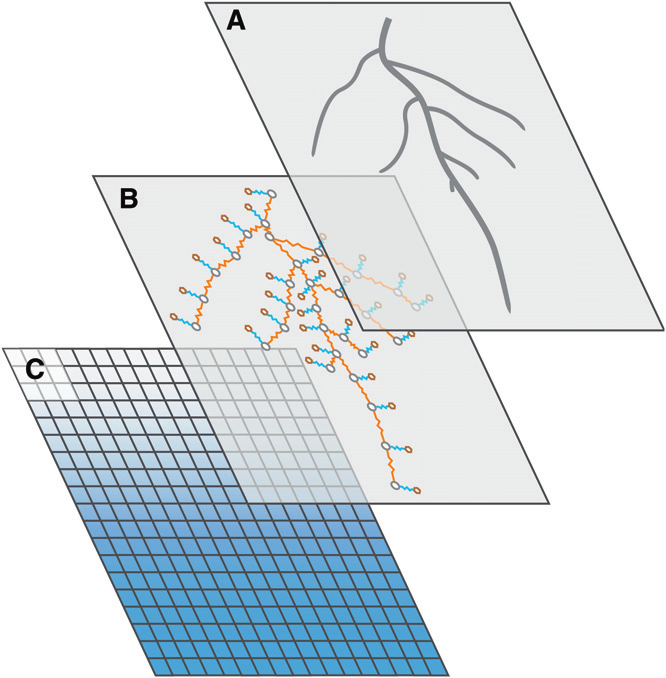
\includegraphics[width=0.5\textwidth]{Image/Properties of the soil root system.png}
\caption{Propriétés du système sol-racine \citep{lobet_plant_2014}}
\label{fig:système sol-racine}
\end{figure}

Ces trois composants sont :

\begin{itemize}
    \item A, l'architecture racinaire : le nombre de racines, leurs longueurs, leurs diamètres, leurs placements, ...
    \item B, l'architecture hydraulique de la racine : les résistances hydrauliques axiales $K_{x}$ (lignes oranges) et radiale $K_{r}$ (lignes bleues), de chaque segment racinaire (cercles gris) ainsi que des éléments du sol (cercles bruns).
    \item C, la distribution d'eau dans le sol.
\end{itemize}

Les caractéristiques du sol présentent donc déjà un grand intérêt.
Premièrement, elles définissent la réserve utile en eau du sol qui correspond à la quantité d’eau que le sol peut absorber et restituer à la plante.
Ensuite, la composition du sol influence le potentiel hydrique du sol et ainsi l'absorption d'eau par les racines.
Le sol définit donc la quantité d'eau disponible pour la plante. 
Ensuite, l'architecture racinaire définit la portée qu'a la plante pour explorer le sol et ainsi rendre accessible l'eau disponible dans le sol.
Finalement, l'anatomie racinaire, permet de quantifier l'entrée ($K_{r}$) et le transport ($K_{x}$) de l'eau jusqu'à la base de la tige.
\newline

La variabilité spatio-temporelle dans laquelle évolue une plante fait que des caractéristiques racinaires (architecturales et anatomiques) "parfaites" sont difficilement concevables.
Dès lors, il est préférable de partir du concept de système racinaire "adapté" à un environnement spécifique.
Les plantes ayant un phénotype plus adapté à la disponibilité des ressources dans l'espace et le temps auront un meilleur accès aux ressources comparé aux autres qui n'ont pas bénéficié de cette coïncidence \citep{lynch_steep_2013}.
Cette notion est formalisée sous le terme d'idéotype.

\subsection{Idéotype racinaire : steep, cheap and deep}

Un idéotype, pour une espèce agricole, est un modèle de plante qui correspond à un environnement donné et pas nécessairement à la plante idéale. 
Ce concept a été proposé par \cite{donald_breeding_1968} comme une nouvelle façon de concevoir la sélection végétale.
\newline 

Steep, cheap and deep (pentu, économe et profond) est un idéotype qui a été proposé pour optimiser la récupération d'eau et d'azote chez le maïs. 
Celui-ci décrit un phénotype avec des caractéristiques racinaires architecturales, anatomiques et physiologiques permettant une meilleure exploitation des couches de sols profondes.
L'idéotype est construit sur base du maïs car c'est, historiquement et encore à ce jour, une culture très répandue. 
Néanmoins, le maïs étant assez exigeant en eau et en azote, cet idéotype peut s'élargir à d'autres cultures ayant un système racinaire fondamentalement similaire (blé, riz, ...) et spécialement le sorgho qui a une architecture et une anatomie racinaire très semblable au maïs \citep{lynch_steep_2013}.
\newline

Steep, cheap and deep part de certains principes pour construire son système racinaire :

\begin{itemize}
    \item L'acquisition des ressources est fortement augmentée lorsque le placement des racines coïncide avec la présence de ressources dans le temps et l'espace.
    \item Le système racinaire représente un coût métabolique non négligeable \citep{kafkafi_respiratory_2002}. Plus le système racinaire est important, plus il est nécessaire de lui allouer des ressources.
    \item L'eau et l'azote sont plus facilement disponibles en profondeur durant la saison de croissance des plantes pour la plupart des sols.
    \item Les racines profondes ont plus de valeurs étant donné qu'elles participent également à l'absorption des ressources proches de la surface alors que les racines peu profondes n'ont pas la faculté d'explorer le sol en profondeur.
    \item L'utilité d'un trait racinaire est évaluée sur base de son coût métabolique et du bénéfice qu'il peut apporter.
\end{itemize}

La figure \ref{fig:steep, cheap and deep} ci-dessous reprend les traits racinaires de l'idéotype cheap, steep and deep dont les principaux seront développés par la suite.

\begin{figure}[ht]
\centering
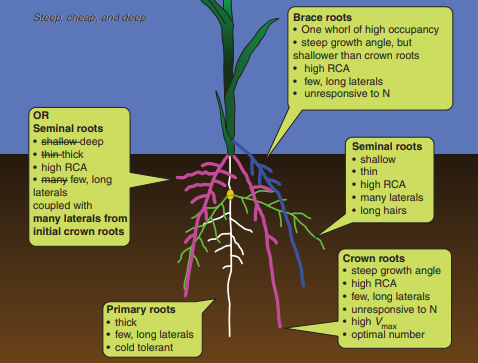
\includegraphics[width=0.75\textwidth]{Image/steep, cheap and deep.png}
\caption{L'idéotype steep, cheap and deep \citep{lynch_steep_2013}}
\label{fig:steep, cheap and deep}
\end{figure}

\subsubsection{Caractéristiques architecturales}

L'architecture du système racinaire (ASR) est une composante principale pour la productivité et la survie de la plante.
Celle-ci définit la quantité de ressources (eau et nutriments) qui est accessible par la plante dans un environnement dynamique et variable. 
L'ASR peut se caractériser par de multiples paramètres et de plus en plus de recherche sont faites afin d'identifier les paramètres clés qui contribuent à une meilleure résilience hydrique.
\newline

\noindent \textbf{La profondeur}

La profondeur est en fait le résultat d'autres paramètres de croissance tel que l'angle de croissance ou encore la vitesse de croissance primaire.
Les couches supérieures du sol sont les plus susceptibles de s'assécher lors d'un épisode de sécheresse. 
Cela est dû à l'évaporation et aux activités biologiques qui sont très importantes dans le haut de la rhizosphère.
Il est alors nécessaire que la plante soit capable de récupérer efficacement de l'eau dans les couches plus profondes du sol afin d'augmenter sa résistance en cas de sécheresse.
Lorsque la profondeur du sol le permet, augmenter la profondeur des racines améliore l'accès à l'eau.
Néanmoins, cette augmentation de la profondeur peut représenter un "gaspillage de photosynthèse" lorsqu'elle n'est pas accompagnée d'une densité de latérales suffisante dans les couches de sols profondes \citep{tardieu_any_2012}.
\newline

\noindent \textbf{La densité de latérale}

Les racines latérales développent considérablement la capacité de la plante à explorer le sol.
Néanmoins, trop de latérales demanderait un métabolisme trop important et réduirait la croissance de la racine mère \citep{lynch_root_2014}.
Plusieurs études ont montré que les coûts métaboliques de l'exploration du sol par les systèmes racinaires sont conséquents et peuvent dépasser 50\% de la photosynthèse quotidienne \citep{kafkafi_respiratory_2002}.
Il est dès lors favorable d'avoir moins mais de plus longues latérales capables d'explorer de plus grands volumes de sol tout en gardant un coût métabolique minimum.
Il serait également préférable que ces latérales soient uniformément distribuées le long de la racine primaire avec toutefois une densité plus élevée dans les couches moyenne et profonde du sol pour améliorer l'absorption en profondeur \citep{wasson_traits_2012}.
\newline

\noindent \textbf{Diamètre}

Un diamètre plus large permet une meilleure pénétration lorsque le sol est dur \citep{bengough_root_2011}.
De plus, il a été observer qu'un diamètre plus large de la racine primaire est lié à un plus grand potentiel de croissance \citep{pages_estimating_2010}.
Une racine ayant un plus grand diamètre est ainsi plus disposée à atteindre les couches plus profondes du sol.
\newline

\noindent \textbf{Tropisme}

En adaptant son système racinaire en fonction de ces stimuli environnementaux, la plante maximise son accès aux ressources et cela participe à augmenter sa résilience dans le cas ou la présence d'eau ou nutriments est limitée.
Les plantes réagissent différemment à ces stimuli et cette capacité d'adaptation peut représenter un atout en condition de manque de ressources.
Il a entre autre été observé par \cite{gul_hydrotropism_2023} que différentes espèces/variétés peuvent avoir un hydrotropisme plus ou moins important illustrant ces différences d'adaptation entre plants.

\subsubsection{Caractéristiques anatomiques}

L'anatomie racinaire impacte l'entrée des ressources dans la plante et l'efficacité avec laquelle elles sont allouées en son sein.
Il est donc intéressant de s'y attarder pour modifier l'architecture hydraulique des racines et ainsi améliorer la résistance au stress.
Un segment racinaire se différencie par sa conduction hydraulique axiale et radiale ainsi que la conductance du chemin le plus court qui le relie à la base de la tige \citep{lobet_plant_2014}.
\citep{wasson_traits_2012} avancent que de plus grandes conductivités axiale et radiale augmentent la capacité de la plante à récupérer et à transporter l'eau contenue dans les sols profonds. 
\newline

\noindent \textbf{Conductivité radiale}

La conductivité radiale permet l'entrée d'eau depuis le sol dans les racines.
Celle-ci est largement influencée par la succession de couches qu'il peut y avoir entre la surface de la racine et le xylème.

\begin{minipage}{0.55\linewidth}
\captionsetup{type=figure,hypcap=true}
\centering
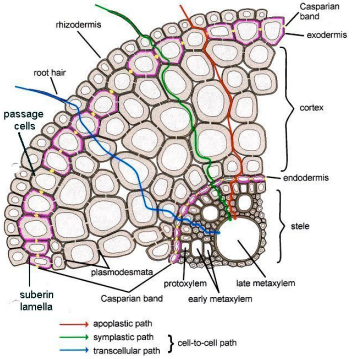
\includegraphics[width=\linewidth]{Image/radial flow.png}
\captionof{figure}{Conductivité radiale \citep{ranathunge_new_2005}.}
\label{fig:radial flow}
\end{minipage}\hfill
\begin{minipage}{0.4\linewidth}
La figure \ref{fig:radial flow} illustre les différentes voies par lesquelles l'eau peut s'infiltrer jusqu'au xylème ainsi que les différentes couches qui composent ces chemins.
La conductivité radiale est largement influencée par la succession de couches, leurs anatomies ainsi que la présence de cadres de Caspary qui sont des structures hydrophobes \citep{yang_drought-induced_2012}.
L'anatomie racinaire est altérée à long terme par les conditions environnementales.
Les structures hydrophobes peuvent, par exemple, être mises en place suite à un épisode de sécheresse \citep{vandeleur_role_2009}.
À court terme, la plante peut également s'adapter aux conditions dans la rhizosphère via la régulation des aquaporines qui peuvent, pour certaines espèces, participer jusqu'à 80\% du flux radial \citep{javot_role_2003}.
\end{minipage} 
\newline

\noindent \textbf{Conductivité axiale}

La conductivité axiale mesure le déplacement de la sève minérale au sein de la plante.
Celle-ci peut, comme la conductivité radiale, être altérée par des mécanismes qui l'influence à long et court terme.
Parmi les caractéristiques qui impactent sur le long terme, on retrouve : la taille, le nombre et la qualité d'interconnexions des vaisseaux de xylème qui sont les conduits du flux axial.
En ce qui concerne l'influence à court terme de la conductivité axiale, les principaux phénomènes sont les embolies causées par des cavitations dans les vaisseaux de xylèmes.
La cavitation intervient lorsque la tension créée dans le xylème par la transpiration des feuilles devient trop importante.
Il se crée alors des bulles de gaz dans le xylème, ce qui rend les vaisseaux concernés hermétiques au passage de l'eau, ce qui limite ainsi les flux d'eau aux autres vaisseaux qui n'ont pas de cavités.
Il a été montré par \cite{delzon_mechanism_2010} que la susceptibilité à la cavitation est liée à la taille des vaisseaux de xylème, à la rugosité des parois et à l'abondance de perforation dans le xylème.
Optimiser ces caractéristiques peut donc participer à réduire les phénomènes de cavitation dans les plantes.
\newline

\noindent \textbf{Root Cortical Aerenchyma (RCA)}

L'aérenchyme est un tissu végétal constitué de cellules séparées par de grandes cavités.
Son intérêt dans les racines a longtemps été réduit à faciliter des transferts gazeux lorsque les plantes font face à l'hypoxie.
Cependant, il est aujourd'hui également considéré que sa présence permet une meilleure exploration des sols par les racines en réduisant leurs coûts métaboliques.
Le RCA réduit les besoins en respirations et en nutriments des tissus racinaires, ce qui permet une plus grande croissance racinaire pour un même coût métabolique.
Sa présence est donc favorable dans des conditions déficitaires en eau bien que l'aérenchyme peut réduire le flux d'eau radiale dans les racines.


\subsubsection{Caractéristiques physiologiques}

La physiologie des plantes joue un rôle crucial dans la capacité des plantes à survivre et à s'adapter à leur environnement.
Les plantes sont capables de s'adapter à leur environnement en réagissant aux stimuli externes qu'elles reçoivent.
La morphologie des poils racinaires, les exsudats racinaires, une augmentation de la croissance racinaire ou encore les différents tropismes sont des mécanismes dont dispose la plante pour modifier son ASR et ainsi répondre aux conditions environnantes \citep{dunbabin_modelling_2013}.
L'architecture et l'anatomie racinaire de la plante découlent donc en partie de la physiologie de la plante.
\newline

Le "root cost of acquisition", qui est plus une conséquence de l'anatomie, l'architecture et la physiologie, mesure essentiellement l'habileté de la plante à acquérir des ressources en fonction de l'investissement mis dans la production de ses racines.
Dans cet idéotype, l'idée est de minimiser le coût énergétique et matériel pour produire les racines tout en maximisant leur disposition à explorer le sol en profondeur et à extraire l'eau nécessaire à la plante.
La présence d'aérenchymes peut, par exemple, améliorer le "coût d'acquisition de ressources" en réduisant le coût métabolique des racines.
De même que la présence de longue latérale bien répartie.
\newline

\subsection{Modélisation des flux hydriques dans les racines}

Modéliser les flux hydriques dans le système sol-plante nécessite l'intervention d'une multitude d'éléments.
Ces éléments sont, pour beaucoup, dynamiques et hétérogènes, ce qui complique l'appréhension du système dans sa globalité.
\cite{passot_connecting_2018} imaginent un réseau qui représente les outils, propriétés et variables d'états nécessaires pour quantifier les interactions entre les différents éléments du système sol-plante.
Ce réseau fait intervenir des procédures expérimentales, des outils informatiques et des données propres aux flux hydriques.
La figure \ref{fig:modelling} représente la partie considérée dans ce travail de ce réseau (le réseau complet est disponible en annexe \ref{an:modelling_full}).
Le réseau réduit est alors compartimenté en fonction de deux "dimensions" et de deux "échelles".
Les flux hydriques peuvent être caractérisés à l'échelle d'un organe ou de la plante.
De plus, il serait également nécessaire de prendre en compte des aspects structurels et fonctionnels.
\newpage

\begin{figure}[ht]
\centering
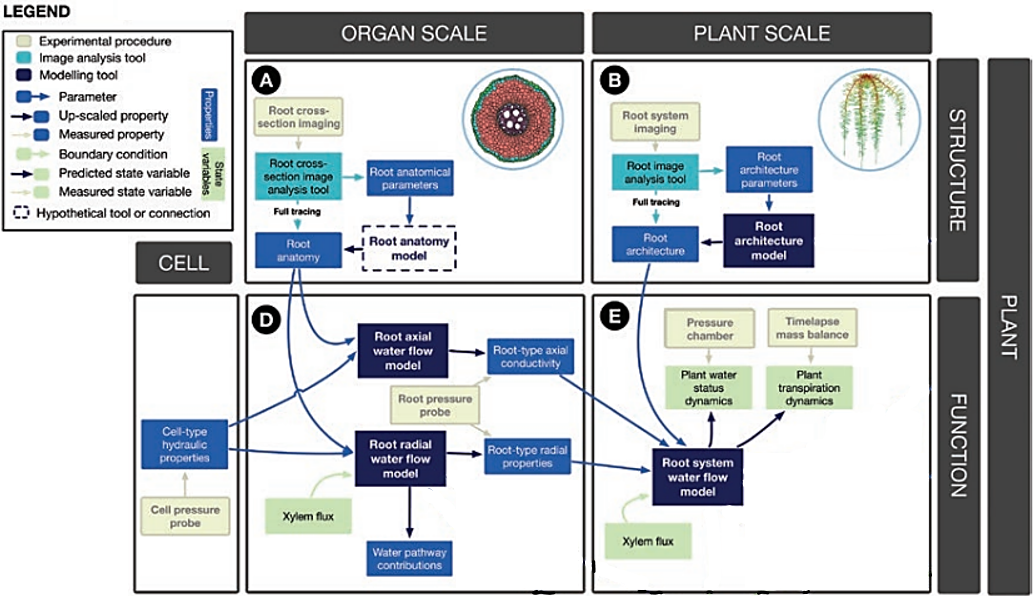
\includegraphics[width=1\textwidth]{Image/modelling_b.png}
\caption{Quantifier les relations hydriques dans le système sol-plante. Réseaux réduit de \cite{passot_connecting_2018}}
\label{fig:modelling}
\end{figure}

\subsubsection{Échantillonnage}
\textbf{Architecture}
\newline
Un problème persistant pour modéliser l'architecture racinaire est l'acquisition de données.
Les données en champs représentent la réalité, mais elles demandent beaucoup de travail et il est difficile d'isoler l'impact d'un facteur précis.
Il est alors nécessaire de procéder en laboratoire ou à l'aide de caractères "proxy" en champs pour quantifier certains traits racinaires spécifiques \citep{wasson_traits_2012}.
Un "proxy" est une mesure racinaire ou aérienne qui serait une conséquence ou du moins corrélée avec le phénotype étudié (exemple : la croissance primaire serait un proxy pour calculer la profondeur de la racine).
\newline

Bien entendu, ces deux méthodes créées un biais dans les données récoltées.
Les expériences en laboratoire permettent d'isoler un facteur en particulier, ce qui permet une étude plus fine de ce facteur.
Mais cela se fait au détriment du réalisme dans lequel se développe le système racinaire.
Les effets de compétitions ou les associations entre organismes sont ignorés, de même que le contenant, le substrat, les nutriments sont définis par l'étude réalisée.
De l'autre côté, l'utilisation d'un proxy sur des données "réalistes" en champs suppose une relation parfaite entre la mesure qui est effectuée et le trait architectural d'intérêt trop difficile à mesurer.
\newline

\textbf{Anatomie}
\newline
L'observation d'échantillon pour l'anatomie racinaire présente plus de facilité que pour l'architecture.
En effet, une section racinaire transversale au microscope permet une vue globale de l'anatomie racinaire d'une racine.
Il n'est alors, dans la majorité des cas, pas trop difficile de parvenir à voir clairement l'ensemble de l'anatomie sans avoir à faire trop de manipulations comme cela peut être le cas pour l'architecture.
Un autre avantage est qu'il n'est pas nécessaire d'observer l'anatomie au cours du temps, un échantillon de fin de culture suffit souvent dans le cas de l'anatomie.

\subsubsection{Modélisation structurelle}

La structure d'un système racinaire peut être décrite à l'échelle de l'organe, ce qui correspond à l'anatomie racinaire, ou à l'échelle de la plante qui correspond alors à l'architecture racinaire.
Dans chacun de ces deux cas, cette structure peut être retracée entièrement sur base d'une observation directe.
Cette méthode s'appelle le "full tracing" et demande énormément de travail, de temps et de rigueur.
Cette méthode présente une alternative qui est la modélisation.
Il suffit alors de tracer une partie de l'anatomie/architecture et d'en extraire des paramètres qui permettent par la suite de reformer, aussi fidèlement que possible, l'ensemble de l'organe ou de la plante.
Chaque modèle se base sur un nombre limité de paramètres requis en input qui sont ainsi considérés comme plus représentatifs d'une architecture/anatomie racinaire.
Les autres caractéristiques sont dans ce cas stochastiques ou construites sur base des inputs.
L'utilisation de tel ou tel modèle demande donc de sélectionner les inputs qui seront considérés.
Cela permet finalement de générer bon nombre d'architectures de systèmes racinaires parfois très contrastés les unes des autres.
\newline

La figure \ref{fig:structure generation}, qui condense la partie structurelle du réseau précédemment présenté (figure \ref{fig:modelling}), illustre la démarche globale permettant la génération de structures racinaires (anatomique ou architecturale).

\begin{figure}[ht]
\centering
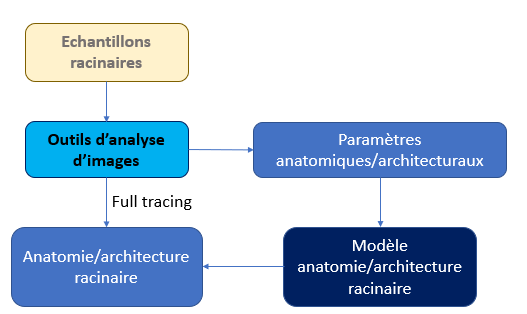
\includegraphics[width=0.5\textwidth]{Image/structure generation.png}
\caption{Génération d'une structure (anatomie ou architecture) de système racinaire}.
\label{fig:structure generation}
\end{figure}

Les données récoltées (de publication préexistante ou d'échantillons racinaire) permettent de mesurer/quantifier des caractéristiques racinaires.
Les caractéristiques considérées comme étant plus déterminantes sont extraites et introduites dans un modèle qui va recréer l'ASR ou l'anatomie sur base de ces quelques caractéristiques.
Finalement, l'architecture/anatomie générée par le modèle devrait correspondre à ce que l'on aurait pu observer empiriquement via le "full tracing" mais qui aurait demandé énormément de rigueur et de travail afin de tout mesurer.

\subsubsection{Modélisation fonctionnelle}

La modélisation fonctionnelle utilise les structures préalablement construites pour quantifier les différents processus de flux hydriques.
Le flux radial ainsi que le flux axial dépendent en partie de l'anatomie racinaire.
Il est donc possible, sur base de celle-ci ainsi que certaines propriétés hydriques (e.g. équation de Hagen-Poiseuille) et modèles (e.g. MECHA), d'estimer le flux radial et le flux axial au niveau d'un segment racinaire.
\newline

Finalement, en récupérant la conductivité axiale ainsi que les propriétés du flux radial, il est possible d'intégrer ces flux à l'ensemble de l'architecture racinaire et ainsi obtenir un modèle pour les flux hydriques dans le système racinaire (e.g.MARSHAL).

\subsection{Sorgho}
Le sorgho est une monocotylédone de la famille des Poaceae qui est cultivée entre mai et octobre.
C'est une plante herbacée annuelle qui peut être cultivée pour ses grains (sorgho grains) ou comme fourrage (sorgho fourrager).
Le sorgho figure, selon la FAO ( l'Organisation des Nations unies pour l'alimentation et l'agriculture), parmi les céréales les plus cultivées dans le monde. 
Celui-ci est à ce jour principalement répandu en Afrique, Asie et Amérique du Sud en raison de sa bonne acclimatation aux climats chauds et arides.
Ses multiples intérêts : alimentation humaine, alimentation animale (fourrage et grain) et application industrielle (agro-carburant, ...) confère au sorgho une certaine importance et sa résilience hydrique pourrait le rendre incontournable au vu des changements climatiques observés.
\newline

En effet, le sorgho est connu pour avoir une grande tolérance face à la sécheresse. Plusieurs causes ont déjà été identifiées pour tenter de comprendre cette résilience telle que :
\begin{itemize}
    \item Fixation du carbone en C4 qui permet de limiter les pertes d'eau par l'ouverture des stomates nécessaire pour la photosynthèse. Les plantes en C4 ont ainsi une meilleure efficience photosynthétique et sont plus adaptées aux climats chaud et sec \citep{shanker_c4_2011}.
    \item Un rapport $\frac{racines}{pousses}$ qui augmente lorsqu'il y a une diminution de l'humidité du sol, ce qui représente un mécanisme de survie face à la sécheresse \citep{mwamahonje_drought_2021}.
    \item L'aptitude "Stay-green" qui représente une bonne adaptation à la sécheresse.
    Celui-ci consiste pour la plante à réduire la taille du couvert à la floraison, ce qui permet d'assurer une disponibilité en eau suffisante pendant le remplissage des grains et ainsi de meilleurs rendements en cas de sécheresse.
    \item Un système racinaire réputé assez profond et étendu.
\end{itemize}
Le sorgho est donc une culture idéale dans les régions où l'eau et les nutriments sont limités. 
En étudiant le système racinaire du sorgho, il serait intéressant de comprendre comment les racines de cette plante participent à la résilience hydrique de la plante.
\newline

Le système racinaire du sorgho est déjà caractérisé de "robuste" et participerait effectivement à faire face aux conditions environnementales difficiles, notamment la pénurie d'eau.
Le schéma \ref{fig:RSA} illustre l'organisation classique du système racinaire des Graminées comme le sorgho.

\begin{figure}[ht]
\centering
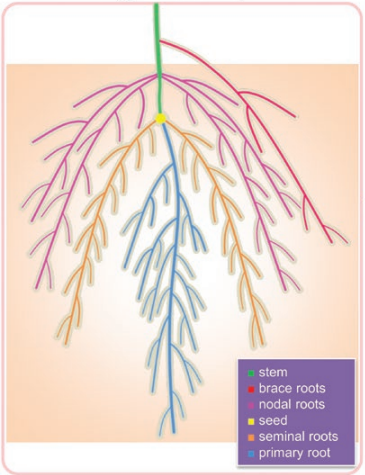
\includegraphics[width=0.5\textwidth]{Image/RSA.png}
\caption{Illustration d'un système racinaire de Graminée \citep{correa_soil_2019}}.
\label{fig:RSA}
\end{figure}

Au début de la germination, le sorgho développe une seule racine primaire qui produit de nombreuses ramifications secondaires.
Le sorgho, contrairement au maïs, ne développe pas de racine séminale en plus de la racine primaire.
Les racines nodales se forment ensuite successivement, prenant la place de la racine séminale qui disparaît progressivement.
Les nœuds souterrains produisent une quantité croissante de racines nodales en fonction de leur position.
Lorsque les racines nodales se développent à partir des nœuds aériens, leur insertion est nettement verticillée \citep{kumar_goyal_how_2021}.
\newline

Plusieurs acteurs de l'agriculture en Belgique s'intéressent depuis quelques années à une potentielle implantation du sorgho dans les régions aux climats tempérés comme en Belgique.
On retrouve, entre autre, le Centre Indépendant de Promotion Fourragère (CIPF).
Le CIPF expérimente et vulgarise différents sujets liés aux cultures de maïs, miscanthus, silphie ou encore le sorgho.
Ainsi, depuis 2013, le CIPF réalise différents tests culturaux sur le sorgho afin d'étudier l'intérêt agronomique que peuvent avoir les différentes variétés.
Il partage ensuite les résultats obtenus dans le but de conseiller/déconseiller une culture de sorgho.